%% 
%% Copyright 2007-2020 Elsevier Ltd
%% 
%% This file is part of the 'Elsarticle Bundle'.
%% ---------------------------------------------
%% 
%% It may be distributed under the conditions of the LaTeX Project Public
%% License, either version 1.2 of this license or (at your option) any
%% later version.  The latest version of this license is in
%%    http://www.latex-project.org/lppl.txt
%% and version 1.2 or later is part of all distributions of LaTeX
%% version 1999/12/01 or later.
%% 
%% The list of all files belonging to the 'Elsarticle Bundle' is
%% given in the file `manifest.txt'.
%% 

%% Template article for Elsevier's document class `elsarticle'
%% with numbered style bibliographic references
%% SP 2008/03/01
%%
%% 
%%
%% $Id: elsarticle-template-num.tex 190 2020-11-23 11:12:32Z rishi $
%%
%%
\documentclass[preprint,12pt]{elsarticle}
%% Use the option review to obtain double line spacing
%% \documentclass[authoryear,preprint,review,12pt]{elsarticle}

%% Use the options 1p,twocolumn; 3p; 3p,twocolumn; 5p; or 5p,twocolumn
%% for a journal layout:
%% \documentclass[final,1p,times]{elsarticle}
%% \documentclass[final,1p,times,twocolumn]{elsarticle}
%% \documentclass[final,3p,times]{elsarticle}
%% \documentclass[final,3p,times,twocolumn]{elsarticle}
%% \documentclass[final,5p,times]{elsarticle}
%% \documentclass[final,5p,times,twocolumn]{elsarticle}

%% For including figures, graphicx.sty has been loaded in
%% elsarticle.cls. If you prefer to use the old commands
%% please give \usepackage{epsfig}

%% The amssymb package provides various useful mathematical symbols
\usepackage{amssymb}
\usepackage{relsize}
\usepackage{array}
\usepackage{caption}
\usepackage{subcaption}
\usepackage{amsmath}
  \DeclareMathOperator*{\argmax}{arg\!max}
  \DeclareMathOperator*{\argmin}{arg\!min}

\newcolumntype{L}[1]{>{\raggedright\let\newline\\\arraybackslash\hspace{0pt}}m{#1}}
\newcolumntype{C}[1]{>{\centering\let\newline\\\arraybackslash\hspace{0pt}}m{#1}}
\newcolumntype{R}[1]{>{\raggedleft\let\newline\\\arraybackslash\hspace{0pt}}m{#1}}
\newcolumntype{M}[1]{>{\centering\arraybackslash}m{#1}}

\usepackage[margin=2.5cm]{geometry}
\usepackage{booktabs}

\usepackage{tikz}
\usepackage{adjustbox}
\usepackage{amsfonts} 

\newsavebox{\mysavebox}

%% The amsthm package provides extended theorem environments
%% \usepackage{amsthm}

%% The lineno packages adds line numbers. Start line numbering with
%% \begin{linenumbers}, end it with \end{linenumbers}. Or switch it on
%% for the whole article with \linenumbers.
%% \usepackage{lineno}

\journal{Neural Networks}

\begin{document}

\begin{frontmatter}

%% Title, authors and addresses

%% use the tnoteref command within \title for footnotes;
%% use the tnotetext command for theassociated footnote;
%% use the fnref command within \author or \address for footnotes;
%% use the fntext command for theassociated footnote;
%% use the corref command within \author for corresponding author footnotes;
%% use the cortext command for theassociated footnote;
%% use the ead command for the email address,
%% and the form \ead[url] for the home page:
%% \title{Title\tnoteref{label1}}
%% \tnotetext[label1]{}
%% \author{Name\corref{cor1}\fnref{label2}}
%% \ead{email address}
%% \ead[url]{home page}
%% \fntext[label2]{}
%% \cortext[cor1]{}
%% \affiliation{organization={},
%%             addressline={},
%%             city={},
%%             postcode={},
%%             state={},
%%             country={}}
%% \fntext[label3]{}

%\title{Signed Saliency Maps}
%\title{The mood of saliency maps: how separating positive and active gradients impact the interpretability  convolutional neural networks}
%\title{The interpretation depends on your mood: considering the sign of gradients to better identify the relevant pixels in saliency maps}
%\title{A matter of attitude: Using positive and active gradients to enhance saliency maps}
%\title{A matter of attitude: Using positive and active gradients to boost saliency maps}
%\title{A matter of attitude: Analysing positive and active gradients to boost saliency maps}
\title{A matter of attitude: Focusing on positive and active gradients to boost saliency maps}
%\title{A matter of attitude: Focusing on positive and active gradients to boost the interpretability/explainability of saliency maps}

%% use optional labels to link authors explicitly to addresses:
%% \author[label1,label2]{}
%% \affiliation[label1]{organization={},
%%             addressline={},
%%             city={},
%%             postcode={},
%%             state={},
%%             country={}}
%%
%% \affiliation[label2]{organization={},
%%             addressline={},
%%             city={},
%%             postcode={},
%%             state={},
%%             country={}}

\author[inst1]{Oscar Llorente\corref{cor1}}
\ead{oscar.llorente.gonzalez@ericsson.com}

\affiliation[inst1]{organization={BMAS SA NDO SW R\&D Unit B, Ericsson},
            addressline={Retama Ed 1 Torre Suecia}, 
            city={Madrid},
            postcode={28045}, 
            state={Madrid},
            country={Spain}}

\author[inst2]{Jaime Boal}
\ead{jaime.boal@iit.comillas.edu}
\author[inst2]{Eugenio F. Sánchez-Úbeda}
\ead{eugenio.sanchez@iit.comillas.edu}

\affiliation[inst2]{organization={Institute for Research in Technology~(IIT), ICAI School of Engineering, Comillas Pontifical University},
            addressline={Santa Cruz de Marcenado, 26}, 
            city={Madrid},
            postcode={28015}, 
            state={Madrid},
            country={Spain}}

\begin{abstract}
%% Text of abstract
Lorem ipsum dolor sit amet, consectetur adipiscing elit, sed do eiusmod tempor incididunt ut labore et dolore magna aliqua. Ut enim ad minim veniam, quis nostrud exercitation ullamco laboris nisi ut aliquip ex ea commodo consequat. Duis aute irure dolor in reprehenderit in voluptate velit esse cillum dolore eu fugiat nulla pariatur. Excepteur sint occaecat cupidatat non proident, sunt in culpa qui officia deserunt mollit anim id est laborum.
\end{abstract}

%%Graphical abstract
%\begin{graphicalabstract}
%
\includegraphics{grabs}
%\end{graphicalabstract}

%%Research highlights
%\begin{highlights}
%\item Research highlight 1
%\item Research highlight 2
%\end{highlights}

\begin{keyword}
%% keywords here, in the form: keyword \sep keyword
eXplainable Artificial Intelligence (XAI) \sep Convolutional Neural Networks \sep Saliency maps \sep Visualization \sep Gradient signs
%% PACS codes here, in the form: \PACS code \sep code
%\PACS 0000 \sep 1111
%% MSC codes here, in the form: \MSC code \sep code
%% or \MSC[2008] code \sep code (2000 is the default)
%\MSC 0000 \sep 1111
\end{keyword}

\end{frontmatter}

%% \linenumbers

%% main text
\section{Introduction}
\label{sec:introduction}
Since the introduction of AlexNet~\cite{krizhevskyImageNetClassificationDeep2012} in the ImageNet~\cite{ImageNet} competition there has been a revolution in the Computer Vision field, where almost in any problem deep learning architectures are the considered the state of the art. However, this type of technology has a big drawback, specially if it is used in sensitive domains, as medicine or autonomous vehicles, its explainability. Due to the high number of parameters (billions) and the complexity of these techniques, it is difficult to explain how a neural network make a certain prediction. To solve this problem, there are two main lines of research:

\begin{itemize}
    \item Building more interpretable models.
    \item Developing techniques to explain the state of the art architectures.
\end{itemize}

There have been attempts to construct these interpretable models for the sensitive domains as in~\cite{singhThinkPositiveInterpretable2022}. However, there are also many other techniques used for Computer Vision problems that offer great results and are not easy to explain, as the classical Convolutional Neural Networks (CNNs)~\cite{lecunConvolutionalNetworksImages}. To explain these other models  several techniques have been developed during the last years. One of the most used types are saliency maps.

Saliency maps were introduced first in~\cite{simonyanDeepConvolutionalNetworks2014} to explain the classification of a neural network based on its derivatives. This type of methods are commonly tested in a multi-class classification problem that can be defined as the following:

\begin{equation}
    \label{eq: cnn output}
    \hat{c} = \argmax_{c \in C}S_c(\boldsymbol{I}),
\end{equation}

\noindent
being $\boldsymbol{I}$ the input image, $C$ the set of all possible classes and $S_c$ the classification score for a certain class $c$. Since usually an image is expressed in rgb format is important to note that $\boldsymbol{I} \in \mathbb{R}^{\text{channels}\, x\, \text{height}\, x\, \text{width}}$. Then, the original saliency map method is expressed as:

\begin{equation}
    \label{eq: 3d saliency map}
    \boldsymbol{M}_{i\, j} = \max_{k} \bigg ( \frac{\partial S_{\hat{c}}}{\partial \boldsymbol{I}_{k\, i\, j}} \bigg ),
\end{equation}

\noindent
being $\boldsymbol{M}$ a 2D map, $k$ an specific channel and, $i$ and $j$, the height and width coordinates, respectively. According to~\cite{simonyanDeepConvolutionalNetworks2014}, the brightest points in a saliency map, i.e., the derivatives with a higher absolute value, are the points that, with a minimum change, affect the class score the most. As it is shown in the previous equation, to derive a single value per pixel, the maximum function over the three pixels is computed. Even though this decision can seem arbitrary, this is the convention that has been followed in every paper about saliency maps.

However, the original saliency maps are very noisy. Therefore, in the following years many variations were suggested to try to improve this visualization and make this noise disappear, as in \cite{springenbergStrivingSimplicityAll2015a, sundararajanAxiomaticAttributionDeep2017, shrikumarNotJustBlack2017}. By these, sharper visualizations were achieved, being these ones more similar to the object in the image and reducing the noise. Unfortunately, in~\cite{adebayoSanityChecksSaliency2018} it was proved that some of these techniques were not showing information about what the neural network has learned, but features from the image, as an edge detector. 

Nevertheless, there is no need of using these techniques to improve the ones from the original saliency maps: more knowledge can be unlocked from the gradients of the neural network without further modifications. First, the sign of the gradients has not been studied in any paper. This sign can have a meaning and a significant impact in the neural network behavior that researchers are trying to understand. Moreover, the type of problem being studied is a multi-class classification problem, and a visualization that tries to explain that, should take into account all these classes and not only the one that is being predicted. In other words, the magnitude of the gradients can have a different meaning depending on whether it is greater or smaller than the gradients for other classes. 

\section{The sign in saliency maps}
\label{sec:the sign in saliency maps}
As pointed out in the last section, there is not any research about the meaning or impact of the sign in saliency maps. The only article that discuss briefly this aspect is~\cite{smilkovSmoothGradRemovingNoise}. In this paper it was explained that the raw value of gradients (without absolute value) is commonly used for MNIST dataset~\cite{MNISTHandwrittenDigit} but not in other datasets as ImageNet. The reason for this is that in the former it produces clearer pictures and in the latter is the opposite. 

However, by taking the absolute value of all the pixels in the saliency map, information can be lost. It is not only valuable knowing which pixels are important but also their meaning. For example, it would be significant, for the explainability field, having a technique that can indicate which zones of the image should be brighter to improve the classification and which ones should be darker. This is in fact the information that the sign can provide. Moreover, if both sets of pixels are combined in the same image without any distinctions between them, they can produce worse explanations. It can seem as if the model is not able to distinguish between zones that should be brighter and others that should be darker, as for example an object in front of a black background. Based on this, two sets of pixels can be distinguished in the image:

\begin{itemize}
    \item Pixels that by increasing their value, the classification score of the predicted class improves since they have a positive value in the saliency map (positive gradient).
    \item Pixels that by decreasing their value, the classification score of the predicted class improves since they have a negative value in the saliency map (negative gradient).
\end{itemize}

Regarding the reason for not using the raw values exposed in~\cite{smilkovSmoothGradRemovingNoise}, it can be due to a high number of 0 values in the saliency map, since when normalized with positives and negatives these pixels will be shining at a medium intensity. To solve this, in this paper the visualization in different images is proposed, having the following new techniques:

\begin{itemize}
    \item Positive saliency maps:
    
    \begin{equation}
        \boldsymbol{M}_{i\, j} = \max_{k} \bigg ( \text{ReLU} \bigg (\frac{\partial S_{\hat{c}}}{\partial \boldsymbol{I}_{k\, i\, j}} \bigg ) \bigg ),
        \label{eq: positive saliency map}
    \end{equation}

    \item Negative saliency maps:
    
    \begin{equation}
      \boldsymbol{M}_{i\, j} = \max_{k} \bigg ( \text{ReLU} \bigg ( - \frac{\partial S_{\hat{c}}}{\partial \boldsymbol{I}_{k\, i\, j}} \bigg ) \bigg ),
      \label{eq: negative saliency map}
  \end{equation}

\end{itemize}

By separating them before taking the absolute value the information about what the pixels mean is not lost. 

\section{Multi-class saliency maps}
\label{sec:multi-class saliency map}
As it was mentioned in Section~\ref{sec:introduction}, the problem being studied is a multi-class classification problem. However, currently all saliency map techniques used the predicted class to compute the derivatives. That does not take into account the information about other classes that the model is predicting. In other words, there can be another gradient, from the derivative respect to other class score, with a higher value than the one respect to the predicted class and the current techniques cannot show that to the user. If it is the case, and the value of this pixel is increased, the classification score for the other class will improve more than the one from the original class, making the prediction of the original class worse, instead of better. The reason for this is that, if the absolute value of all gradients is taken, there cannot be any comparison with the gradients of other classes, since there is no information anymore that can indicate what that a gradient is higher or lower than another means.

However, going further in the analysis started in the last section about the sign allows to compare the gradients of the predicted class and the other ones. In fact, it improves the previous definitions about the different sets of pixels identified in the last section (positive and negative saliency maps):

\begin{itemize}
    \item Pixels that by increasing their value the classification score for the predicted class will improve more that the score from any other class. Since now other classes are taken into account, only the pixels that have a higher gradient with respect to the predicted class than with respect to any other class, will improve the classification if their value is increased.
    \item Analogously, the pixels that by decreasing their value classification score for the predicted class will improve more that the score from any other class, are only the ones that have a lower gradient with respect to the predicted class than with respect to any other class.
\end{itemize}

Therefore, by comparing the saliency maps for the different classes the information about the two sets mentioned before can be extracted. Two new techniques are proposed to represent this:

\begin{itemize}
    \item Active saliency map (increasing them improves the classification score from the original prediction):
    
    \begin{equation}
      \boldsymbol{M}_{i\, j} = \max_{k}
        \begin{cases}
            \frac{\partial S_{\hat{c}}}{\partial \boldsymbol{I}_{k\, i\, j}}, & \frac{\partial S_{\hat{c}}}{\partial \boldsymbol{I}_{k\, i\, j}} = \argmax_{c \in C}\frac{\partial S_{c}}{\partial \boldsymbol{I}_{k\, i\, j}} \\
            0, & \text{otherwise}
        \end{cases}
        \label{eq: active saliency map}
    \end{equation}

    \item Inactive saliency map (decreasing them improves the classification score from the original prediction):
    
    \begin{equation}
      \boldsymbol{M}_{i\, j} = \max_{k}
        \begin{cases}
            \frac{\partial S_{\hat{c}}}{\partial \boldsymbol{I}_{k\, i\, j}}, & \frac{\partial S_{\hat{c}}}{\partial \boldsymbol{I}_{k\, i\, j}} = \argmin_{c \in C}\frac{\partial S_{c}}{\partial \boldsymbol{I}_{k\, i\, j}} \\
            0, & \text{otherwise}
        \end{cases}
        \label{eq: inactive saliency map}
    \end{equation}

\end{itemize}

Note that, both type of methods, positive and negative saliency maps, and active and inactive saliency maps, pursue the same purpose. Positive and active try to find the pixels that by being brighter, increase the confidence of the original classification. Analogously, negative and inactive try to find the pixels that by being darker, also increase the confidence of the original classification.

Positive and negative take into account the sign, which is a significant improvement from the original saliency maps. Active and inactive can be seen as a step further, taking into account also the other classes. Even so, positive and negative can also provide information about which pixels increase the score of the predicted class, even though another score is increasing more. This information can also help the user understand how the class scores of the model works.

\section{Experiments}
\label{sec:experiments}
In this section the new proposed techniques will be evaluated qualitatively and quantitatively. With this purpose, a certain methodology was followed. First, two datasets are used to study the new methods, {CIFAR-10}~\cite{CIFAR10CIFAR100Datasets} and Imagenette~\cite{Imagenette2022}. The first one is a commonly used dataset for image classification and also for explainability. The second one is a subset of 10 classes of ImageNet. It is used this subset instead of the original ImageNet due to computing restrictions of hardware. Then, for CIFAR-10 two model will be used. The first is a CNN model based in a max-pooling, several layers for CNNs, an average-pooling and a final linear layer. The second one is the classical ResNet-18~\cite{heDeepResidualLearning2016}. Both model will be trained from scratch. On the other hand, for Imagenette, in addittion to these two models, a pre-trained version of the ResNet-18 and of the ConvNeXt~\cite{liuConvNet2020s2022} will be used. They were all trained with a learning rate of $0.001$ and the AdamW optimizer for 50 epochs. The results of the test set are the following:

\begin{table}[ht]
  \centering
  \small
  \caption{Test set accuracy.}
  \label{tab: training results}
  \begin{tabular}{L{6cm}C{2cm}C{2cm}}
    \toprule
    {} & CIFAR-10 & Imagenette \\
    \midrule
    Basic CNN & 0.6307 & 0.6205 \\
    ResNet-18  & 0.7569 & 0.8357 \\
    ResNet-18 pre-trained  & - & 0.9733 \\
    ConvNext pre-trained & - & 0.9932 \\
    \bottomrule
  \end{tabular}
\end{table}

\subsection{Qualitative evaluation}

Following the same approach that can be found in the literature of saliency maps, first the techniques will be visually evaluated. In several papers, as in \cite{simonyanDeepConvolutionalNetworks2014}, \cite{springenbergStrivingSimplicityAll2015a}, \cite{smilkovSmoothGradRemovingNoise} or \cite{sundararajanAxiomaticAttributionDeep2017}, the different techniques were compared based on a visual inspection. 

\begin{figure}[ht]
  \centering
  \footnotesize
  \newcommand{\scale}{0.28}
  \setlength{\tabcolsep}{2pt}
  \begin{tabular}{cccccc}
  Image & Original & Positive & Negative & Active & Inactive \\
  
  \includegraphics[scale=\scale]{../visualizations/images/examples/cifar10/cnn_False/1.png} &
  \includegraphics[scale=\scale]{../visualizations/images/saliency_maps/saliency_map/cifar10/cnn_False/1.png} & 
  \includegraphics[scale=\scale]{../visualizations/images/saliency_maps/positive_saliency_map/cifar10/cnn_False/1.png} & 
  \includegraphics[scale=\scale]{../visualizations/images/saliency_maps/negative_saliency_map/cifar10/cnn_False/1.png} & 
  \includegraphics[scale=\scale]{../visualizations/images/saliency_maps/active_saliency_map/cifar10/cnn_False/1.png} & 
  \includegraphics[scale=\scale]{../visualizations/images/saliency_maps/inactive_saliency_map/cifar10/cnn_False/1.png} \\
  
  \includegraphics[scale=\scale]{../visualizations/images/examples/cifar10/cnn_False/2.png} &
  \includegraphics[scale=\scale]{../visualizations/images/saliency_maps/saliency_map/cifar10/cnn_False/2.png} & 
  \includegraphics[scale=\scale]{../visualizations/images/saliency_maps/positive_saliency_map/cifar10/cnn_False/2.png} & 
  \includegraphics[scale=\scale]{../visualizations/images/saliency_maps/negative_saliency_map/cifar10/cnn_False/2.png} & 
  \includegraphics[scale=\scale]{../visualizations/images/saliency_maps/active_saliency_map/cifar10/cnn_False/2.png} & 
  \includegraphics[scale=\scale]{../visualizations/images/saliency_maps/inactive_saliency_map/cifar10/cnn_False/2.png} \\
  \end{tabular}
  \caption{Comparison saliency maps CNN CIFAR-10.}
  \label{fig: comparison saliency maps cnn cifar10}
\end{figure}

\begin{figure}[ht]
  \centering
  \footnotesize
  \newcommand{\scale}{0.28}
  \setlength{\tabcolsep}{2pt}
  \begin{tabular}{cccccc}
  Image & Original & Positive & Negative & Active & Inactive \\
  
  \includegraphics[scale=\scale]{../visualizations/images/examples/imagenette/resnet18_True/8.png} &
  \includegraphics[scale=\scale]{../visualizations/images/saliency_maps/saliency_map/imagenette/resnet18_True/8.png} & 
  \includegraphics[scale=\scale]{../visualizations/images/saliency_maps/positive_saliency_map/imagenette/resnet18_True/8.png} & 
  \includegraphics[scale=\scale]{../visualizations/images/saliency_maps/negative_saliency_map/imagenette/resnet18_True/8.png} & 
  \includegraphics[scale=\scale]{../visualizations/images/saliency_maps/active_saliency_map/imagenette/resnet18_True/8.png} & 
  \includegraphics[scale=\scale]{../visualizations/images/saliency_maps/inactive_saliency_map/imagenette/resnet18_True/8.png} \\
  
  \includegraphics[scale=\scale]{../visualizations/images/examples/imagenette/resnet18_True/3.png} &
  \includegraphics[scale=\scale]{../visualizations/images/saliency_maps/saliency_map/imagenette/resnet18_True/3.png} & 
  \includegraphics[scale=\scale]{../visualizations/images/saliency_maps/positive_saliency_map/imagenette/resnet18_True/3.png} & 
  \includegraphics[scale=\scale]{../visualizations/images/saliency_maps/negative_saliency_map/imagenette/resnet18_True/3.png} & 
  \includegraphics[scale=\scale]{../visualizations/images/saliency_maps/active_saliency_map/imagenette/resnet18_True/3.png} & 
  \includegraphics[scale=\scale]{../visualizations/images/saliency_maps/inactive_saliency_map/imagenette/resnet18_True/3.png} \\
  \end{tabular}
  \caption{Comparison saliency maps ResNet-18 Imagenette.}
  \label{fig: comparison saliency maps resnet18 imagenette}
\end{figure}

One trend in the mentioned article is to just show some examples of the visualization to make the comparison. However, in none of them is explained how these examples are obtained. Therefore, it could be the case that the visualization is better for a certain class or example. To solve this problem in this paper a correct example for each class from the test is randomly selected. These images are shown in~\ref{sec:signed saliency map examples}. Here, two examples can be observed in Figure~\ref{fig: comparison saliency maps cnn cifar10} and Figure~\ref{fig: comparison saliency maps resnet18 imagenette}.

From the comparison it can be appreciated that the proposed techniques reduce the noise of the original saliency maps, producing sharper visualization. The shape of the objects that the neural network is classifying are is clearer and there is a higher level of detail. However, and even though this evaluation is the common approach in the literature, it does not prove that sharper or less noisy visualizations are better. It could be the case that a noisier visualization is more faithful to what the neural network has learned. Because of this, a quantitative evaluation has been done.

\subsection{Quantitative evaluation}

Even though historically the evaluation of saliency maps has been qualitative, there have been efforts to try to formulate metrics to measure the effectiveness of these techniques, as in~\cite{petsiukRISERandomizedInput},~\cite{hookerBenchmarkInterpretabilityMethods2019} or~\cite{anconaBetterUnderstandingGradientbased2018}. While in~\cite{anconaBetterUnderstandingGradientbased2018} it is studied a desirable property of explainability techniques, in~\cite{petsiukRISERandomizedInput} and~\cite{hookerBenchmarkInterpretabilityMethods2019} the objective is to formulate a metric that could indicate which technique is better. 

Specifically,~\cite{petsiukRISERandomizedInput} proposed a metric called deletion that deletes pixels in descending order of importance (according to the explainability technique) and recomputes the probability of the correct output for each fraction of deleted pixels. For the mentioned deletion researchers fixed the values of these pixels to a constant, as black or gray, or to random noise. 

In~\cite{hookerBenchmarkInterpretabilityMethods2019} it was proposed a variation of the deletion metric. In this paper it was explained that it was necessary to retrain the model for each portion of deleted pixels to maintain the same distribution in the training set and the test set, where the explainability technique was being measured. However, in the retraining, the model can learn new other things, so the metric is not measuring how well the explainability technique represents what the neural network has learned because the information used by the model to classify can be different now.

\begin{figure}[p]
    \centering
    \subfloat[CIFAR-10 CNN]{\includegraphics[width=0.475\textwidth]{../visualizations/graphs/cifar10/cnn_False/val/0.pdf}} \hfill
    \subfloat[CIFAR-10 ResNet-18]{\includegraphics[width=0.475\textwidth]{../visualizations/graphs/cifar10/resnet18_False/val/0.pdf}} \\
    \subfloat[Imagenette CNN]{\includegraphics[width=0.475\textwidth]{../visualizations/graphs/imagenette/cnn_False/val/0.pdf}} \hfill
    \subfloat[Imagenette ResNet-18]{\includegraphics[width=0.475\textwidth]{../visualizations/graphs/cifar10/resnet18_False/val/0.pdf}} \\
    \subfloat[Imagenette ResNet-18 pre-trained]{\includegraphics[width=0.475\textwidth]{../visualizations/graphs/imagenette/resnet18_True/val/0.pdf}} \hfill
    \subfloat[Imagenette ConvNeXt pre-trained]{\includegraphics[width=0.475\textwidth]{../visualizations/graphs/imagenette/convnext_True/val/0.pdf}} \\
    \caption{Black-Deletion Benchmark.}
    \label{fig: black-deletion benchmark}
\end{figure}

\begin{figure}[p]
    \centering
    \subfloat[CIFAR-10 CNN]{\includegraphics[width=0.475\textwidth]{../visualizations/graphs/cifar10/cnn_False/val/1.pdf}} \hfill
    \subfloat[CIFAR-10 ResNet-18]{\includegraphics[width=0.475\textwidth]{../visualizations/graphs/cifar10/resnet18_False/val/1.pdf}} \\
    \subfloat[Imagenette CNN]{\includegraphics[width=0.475\textwidth]{../visualizations/graphs/imagenette/cnn_False/val/1.pdf}} \hfill
    \subfloat[Imagenette ResNet-18]{\includegraphics[width=0.475\textwidth]{../visualizations/graphs/cifar10/resnet18_False/val/1.pdf}} \\
    \subfloat[Imagenette ResNet-18 pre-trained]{\includegraphics[width=0.475\textwidth]{../visualizations/graphs/imagenette/resnet18_True/val/1.pdf}} \hfill
    \subfloat[Imagenette ConvNeXt pre-trained]{\includegraphics[width=0.475\textwidth]{../visualizations/graphs/imagenette/convnext_True/val/1.pdf}} \\
    \caption{White-Deletion Benchmark.}
    \label{fig: white-deletion benchmark}
\end{figure}

Going back to the deletion metric, its problem is that the value of a pixel cannot be deleted, because for a neural network any value can have some meaning, including the black, the gray or noise. Then, the value introduced can affect different pixels in different ways, introducing unknown biases. However, the separation in two different sets of pixels, the ones that should be brighter (positive and active saliency maps) to improve the classification score of the original predictions and the ones that should be darker (negative and inactive saliency maps), opens the door to implement the deletion technique knowing what the introduced value means. In this paper the two proposed metrics are called black-deletion and white-deletion.

First, the new techniques give the user the two different sets of pixels (should be brighter and should be darker). Since increasing the value (making them brighter) of some of them improves the classification score of the predicted classes, putting them to zero (black-deletion) should harm severely the original classification. Analogously, putting the pixels that should be darker to improve the original classification to one (white deletion) should show also harm severely the original classification. Therefore, black-deletion will help to measure the effect of positive and active salience maps, while white deletion will be used to measure negative and inactive salience maps. Both metrics will measure the change in the predicted classes with respect to the original classification (something that here has been called allegiance) for the following fractions of deleted pixels: [0.03, 0.05, 0.07, 0.1, 0.2, 0.3, 0.4, 0.5, 0.6, 0.7, 0.8, 0.9]. The interval to measure the deletion is 10\%, since based on the literature~\cite{hookerBenchmarkInterpretabilityMethods2019} it a common interval, with a higher level of detail at the beginning to show the sharp decrease in the first deletions. These can be appreciated in Figure~\ref{fig: black-deletion benchmark} and Figure~\ref{fig: white-deletion benchmark}. 

In the graphs it can be seen that the behavior is the expected, meaning that the selection of positive, negative, active and inactive gradients worked. As expected, the decrease in allegiance for black-deletion is greater for active and positive than for the original saliency map. Analogously, the decrease in allegiance for white-deletion is greater for inactive and negative saliency maps than for the original ones. This proves that the pixels identified.

\begin{table}
  \centering
  \small
  \caption{AUC for black deletions in saliency maps.}
  \label{tab:auc for black deletions in saliency maps}
  \begin{tabular*}{\textwidth}{L{2cm} @{\extracolsep{\fill}} *{8}{c}}
    \toprule
    {} & \multicolumn{2}{c}{CIFAR-10} & \multicolumn{4}{c}{Imagenette} \\
    \cline{2-3} \cline{4-7}
    {} & CNN & ResNet-18 & CNN & ResNet-18 & ResNet-18 pre-trained & ConvNeXt\\  
    \midrule
    Original & 0.23 & 0.23 & 0.24 & 0.26 & 0.28 & 0.49 \\
    Positive & 0.14 & 0.11 & 0.12 & 0.14 & 0.21 & 0.37 \\
    Active   & 0.15 & 0.11 & 0.16 & 0.14 & 0.24 & 0.39 \\ 
    \bottomrule
  \end{tabular*}
\end{table}

\begin{table}
  \centering
  \small
  \caption{AUC for white deletions in saliency maps.}
  \label{tab:auc for white deletions in saliency maps}
  \begin{tabular*}{\textwidth}{L{2cm} @{\extracolsep{\fill}} *{8}{c}}
    \toprule
    {} & \multicolumn{2}{c}{CIFAR-10} & \multicolumn{4}{c}{Imagenette} \\
    \cline{2-3} \cline{4-7}
    {} & CNN & ResNet-18 & CNN & ResNet-18 & ResNet-18 pre-trained & ConvNeXt\\  
    \midrule
    Original & 0.21 & 0.22 & 0.21 & 0.23 & 0.26 & 0.46 \\
    Negative & 0.14 & 0.12 & 0.11 & 0.18 & 0.20 & 0.37 \\ 
    Inactive & 0.15 & 0.12 & 0.14 & 0.16 & 0.23 & 0.42 \\
    \bottomrule
  \end{tabular*}
\end{table}

An important thing to note is that in the graphs it can be seen that for active and inactive saliency maps there is almost no change after 50\% of the pixels have been deleted. The reason for this is that in the active and inactive there are a lot of pixels that are black (because its derivative with respect to the original predicted class is not greater (active) or lower (inactive) than for any other class). Therefore, after all the pixels from the active and inactive saliency maps are deleted there is no change since the pixels that have zero value in the saliency maps were ignored in the deletion (deleting a pixel that does not belong to the saliency map variant does not give us any information). The same happens for the positive and negative later, around 80\%, showing that there are more pixels with positive and negative derivatives, than pixels with a derivative higher or lower with respect to the original class than for any other class.

To give concrete numbers, the area under the curve was also calculated and showed in Table~\ref{tab:auc for black deletions in saliency maps} for black-deletion and in Table~\ref{tab:auc for white deletions in saliency maps} for white-deletion. The intuition of what would happen in the experiments was correct and it has been shown that the new proposed method help the user in identifying pixels that, by being brighter or darker, help the confidence of original predicted classes. However, although the improvement over the original saliency map is clear, it is surprising how positive and negative sometimes work better than active and inactive. The main reason for this could be that these metrics are still not perfect, since the value used for the deletion are the extreme values, and pixels that may improve the classification by being brighter or darker, but that it is not the same that putting their value to white or black. However, from all the possible values to choose, we find most reasonable use the darkest and the brightest value since any pixel can be darker and brighter than them, respectively. Even so, it is still better than the other metrics use in the literature since it introduces a know alteration in the image instead of an unknown one.

Note that every computation shown in this section is based on the test dataset. To see the ones from the training, that have similar results, go to Appendix~\ref{sec:black-deletion and white-deletion for training set}.


\section{Conclusion and future work}
\label{sec:conclusions and future research}
To sum up, in this paper it has been shown that there is more information hidden in the gradients, both in the sign of the gradients and in the gradients of other classes. This paper is the first study that takes into account the sign and the other classes in the explainability, which seem to be crucial for extracting all the information contained in saliency maps. Therefore, it is not necessary to create complicated techniques to create a sharper visualization that shows what the model is looking when it is classifying. Moreover, this can be the starting point of a reformulation of all saliency variants, since it can produce improvements in all the techniques that are based on the gradients. However, this is out of the scope of this article.

Another contribution worth of mentioning is that taking into account the sign or the other classes allows comparing different techniques with the proposed metric, black-deletion and white-deletion. These metrics are the first benchmark that introduces an alteration knowing its meaning, instead of introducing an unknown bias. Therefore, they can also be used to compare more faithfully which are the best saliency techniques. We leave these for future research.


\bibliographystyle{elsarticle-num} 
{\small\bibliography{cas-refs}}

\appendix

\section{Signed saliency map examples}
\label{sec:signed saliency map examples}
In this appendix the examples for each technique will be showed for all the combinations:

\section{Black-Deletion and White-Deletion for Trainning set}
\label{sec:black-deletion and white-deletion for training set}

% \begin{figure}[p]
%   \centering
%   \footnotesize
%   \newcommand{\scale}{0.25}
%   \setlength{\tabcolsep}{2pt}
%   \begin{tabular}{cccccc}
%   Image & Original & Positive & Negative & Active & Inactive \\
  
%   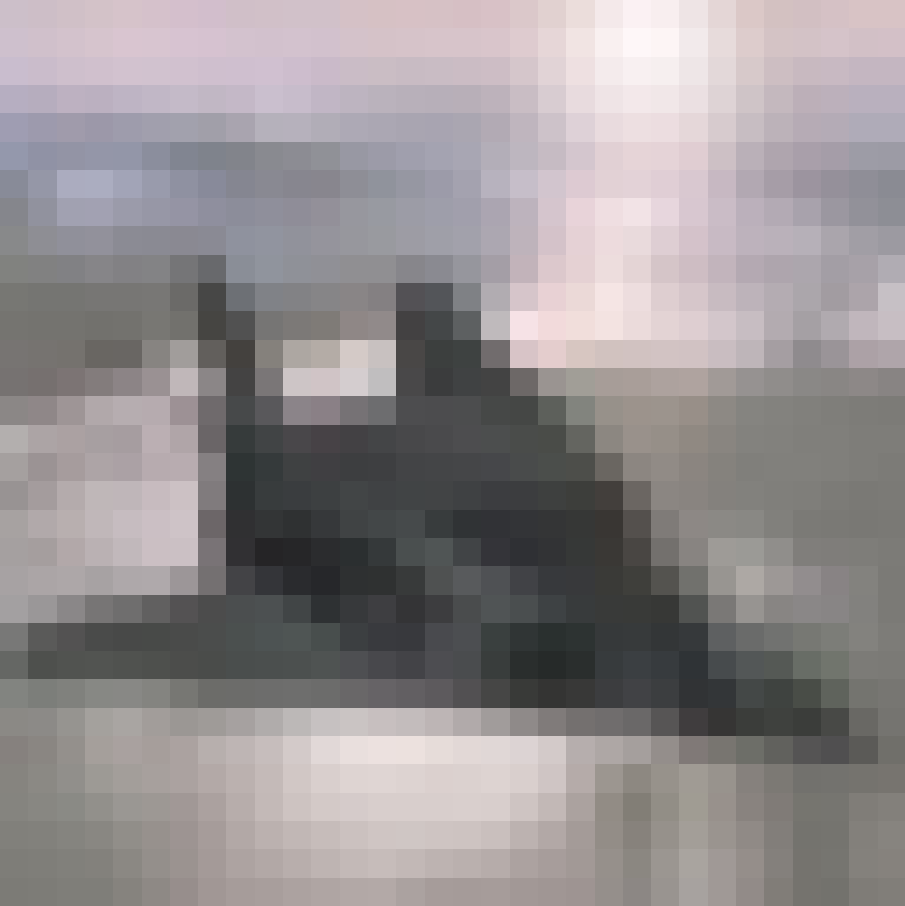
\includegraphics[scale=\scale]{../visualizations/examples/cifar10/cnn/images/0.png} &
%   \includegraphics[scale=\scale]{../visualizations/examples/cifar10/cnn/saliency_map/0.png} & 
%   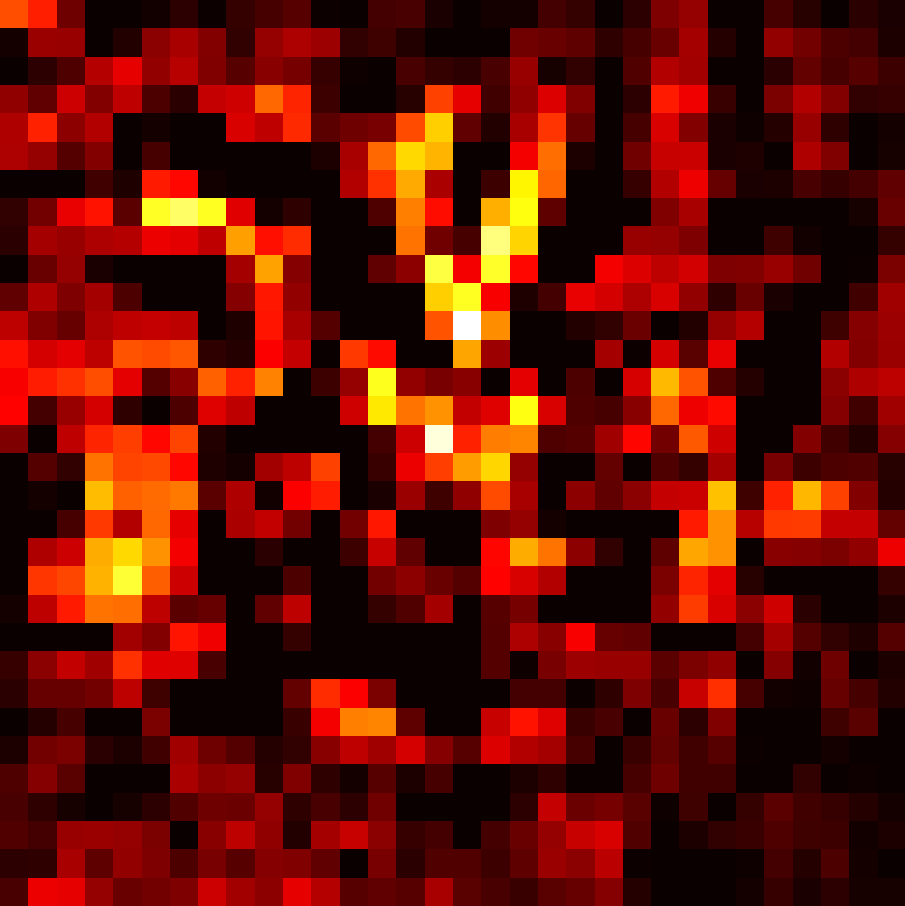
\includegraphics[scale=\scale]{../visualizations/examples/cifar10/cnn/positive_saliency_map/0.png} & 
%   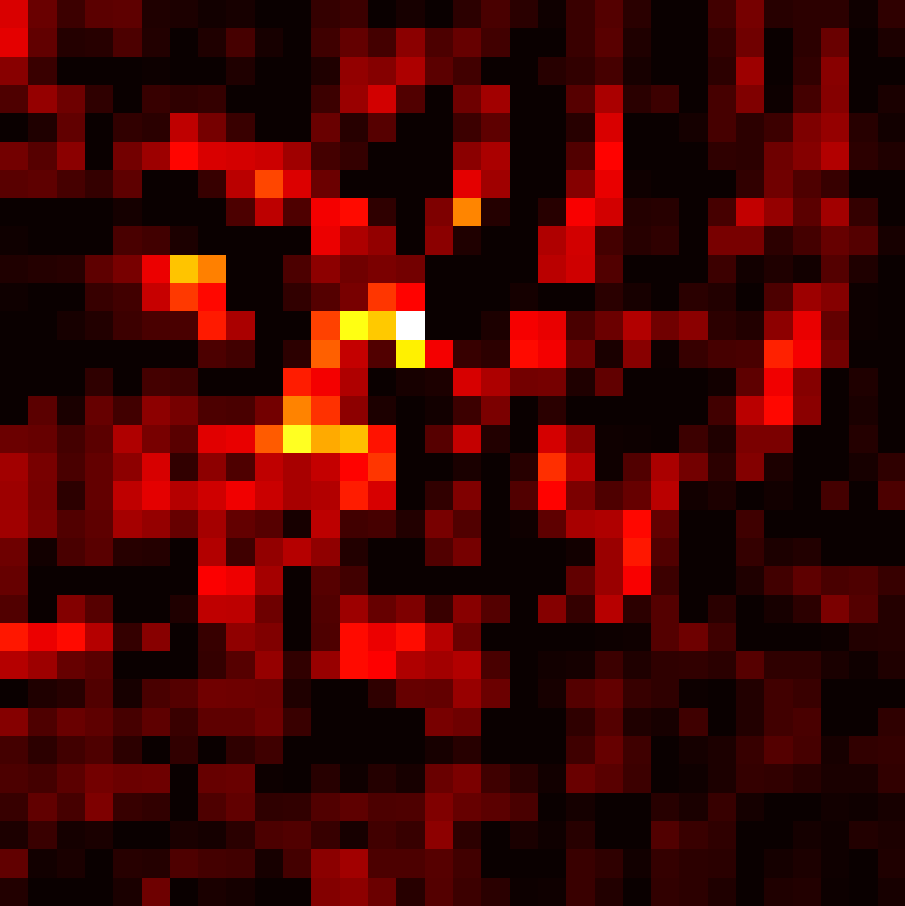
\includegraphics[scale=\scale]{../visualizations/examples/cifar10/cnn/negative_saliency_map/0.png} & 
%   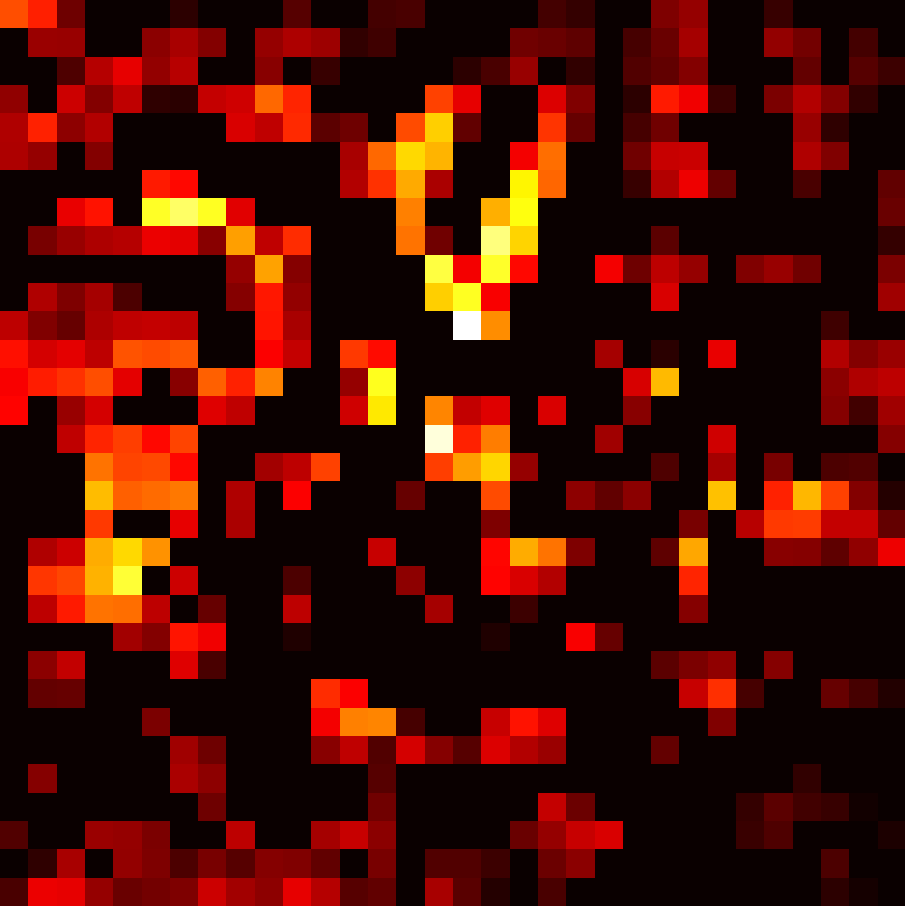
\includegraphics[scale=\scale]{../visualizations/examples/cifar10/cnn/active_saliency_map/0.png} & 
%   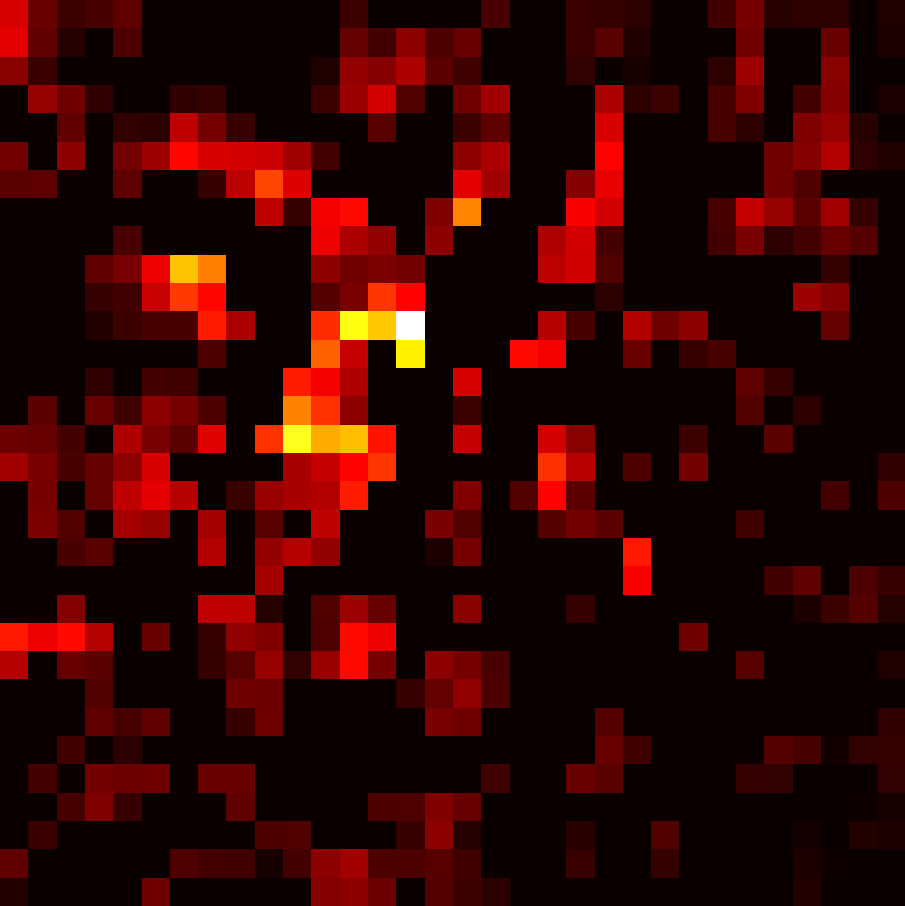
\includegraphics[scale=\scale]{../visualizations/examples/cifar10/cnn/inactive_saliency_map/0.png} \\
  
%   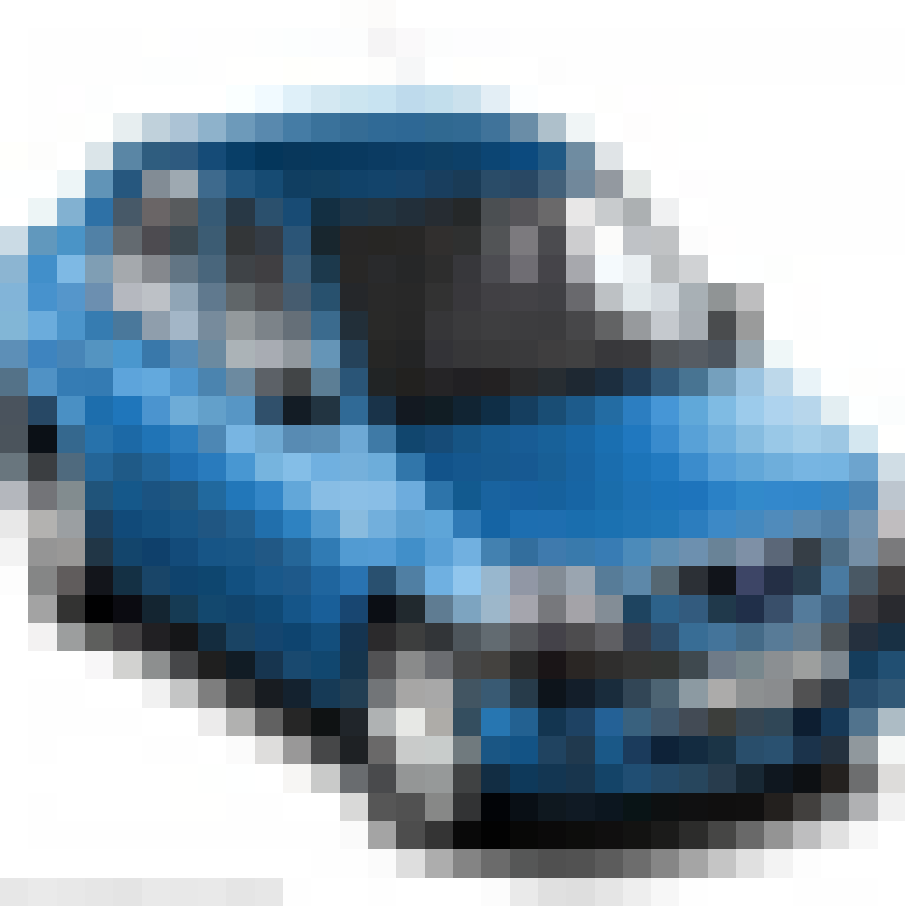
\includegraphics[scale=\scale]{../visualizations/examples/cifar10/cnn/images/1.png} &
%   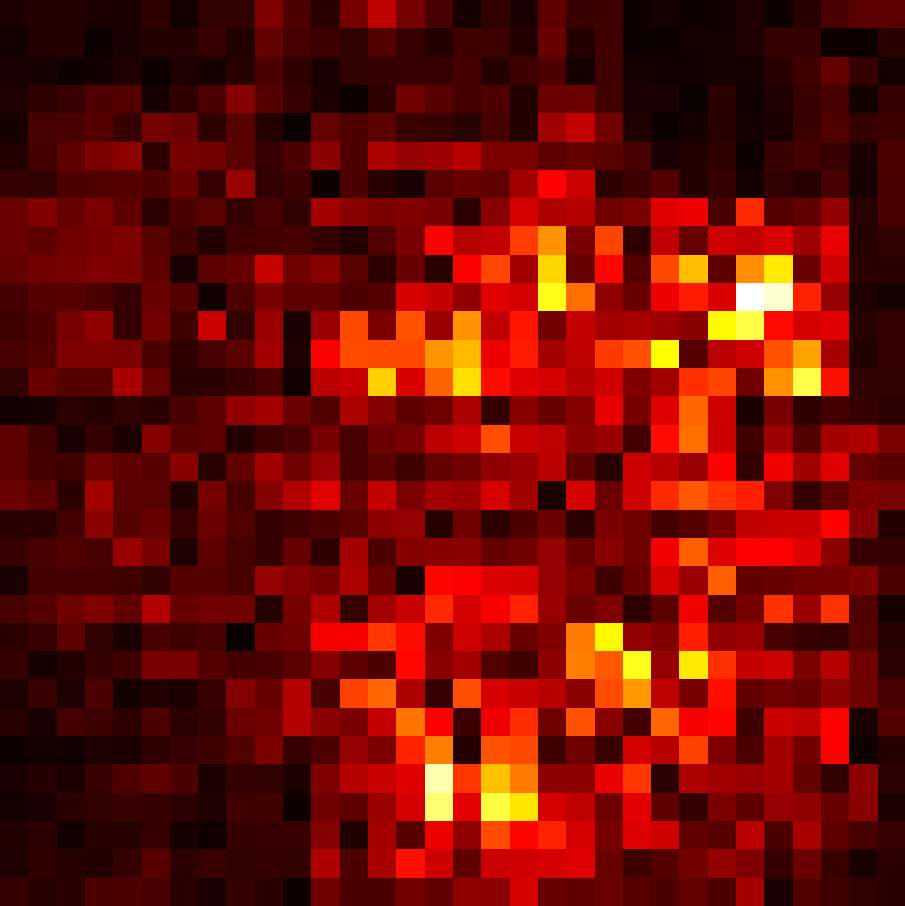
\includegraphics[scale=\scale]{../visualizations/examples/cifar10/cnn/saliency_map/1.png} & 
%   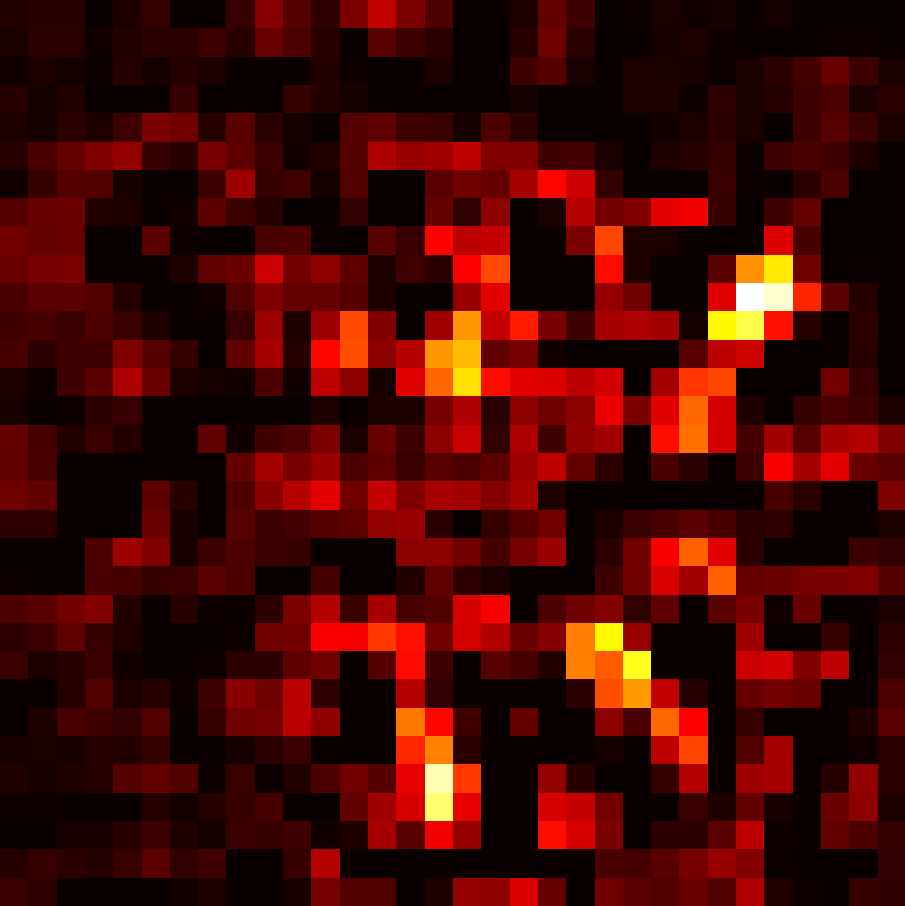
\includegraphics[scale=\scale]{../visualizations/examples/cifar10/cnn/positive_saliency_map/1.png} & 
%   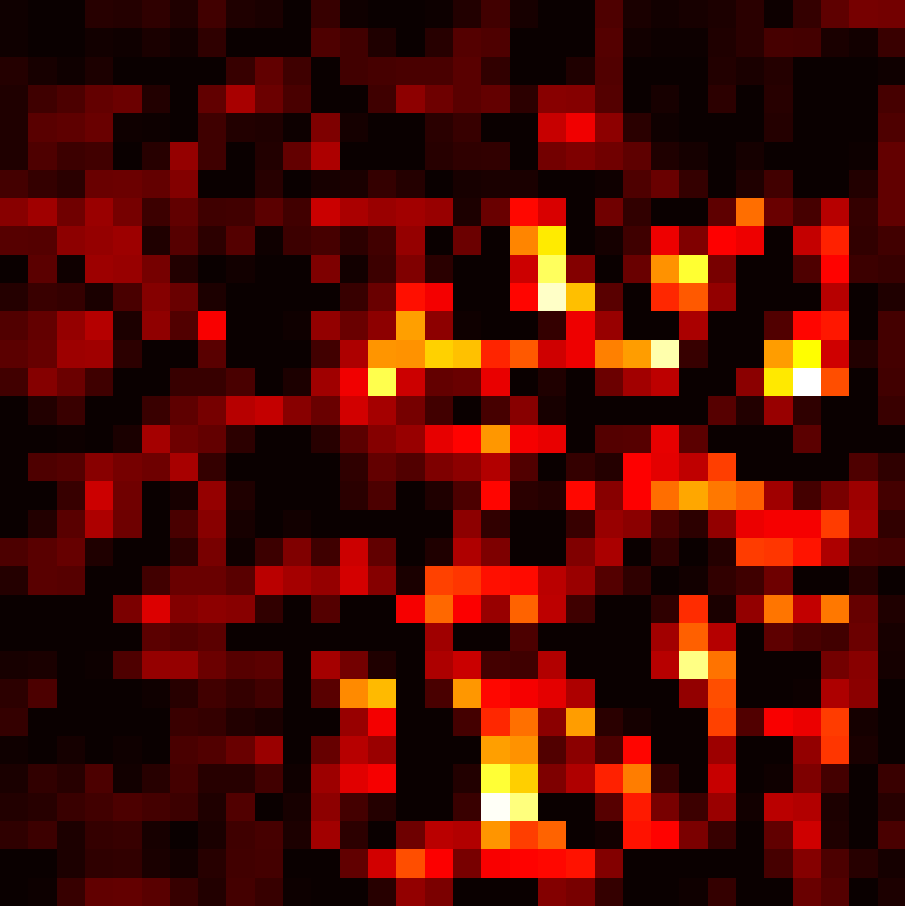
\includegraphics[scale=\scale]{../visualizations/examples/cifar10/cnn/negative_saliency_map/1.png} & 
%   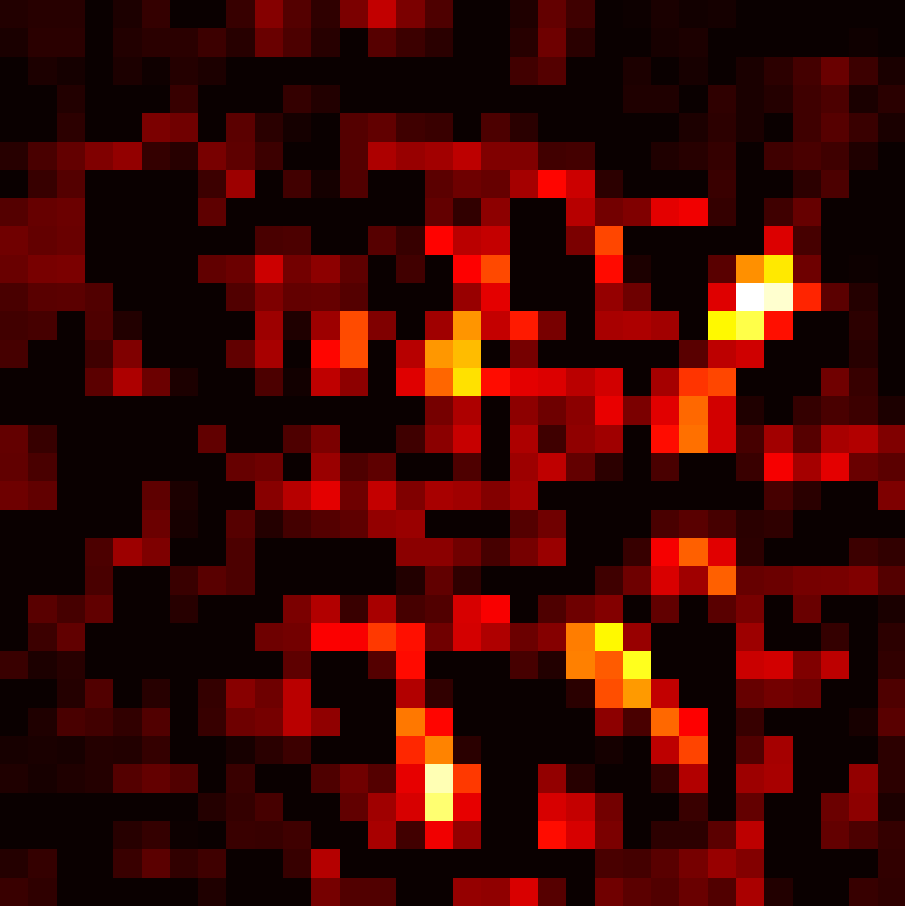
\includegraphics[scale=\scale]{../visualizations/examples/cifar10/cnn/active_saliency_map/1.png} & 
%   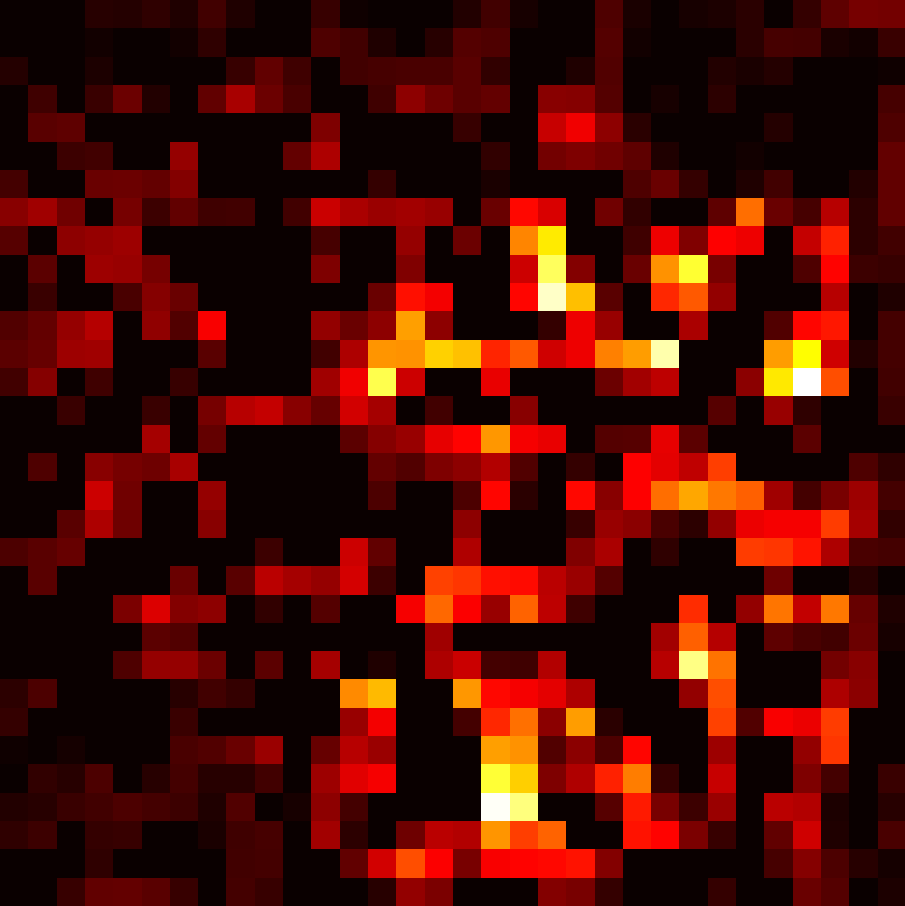
\includegraphics[scale=\scale]{../visualizations/examples/cifar10/cnn/inactive_saliency_map/1.png} \\
  
%   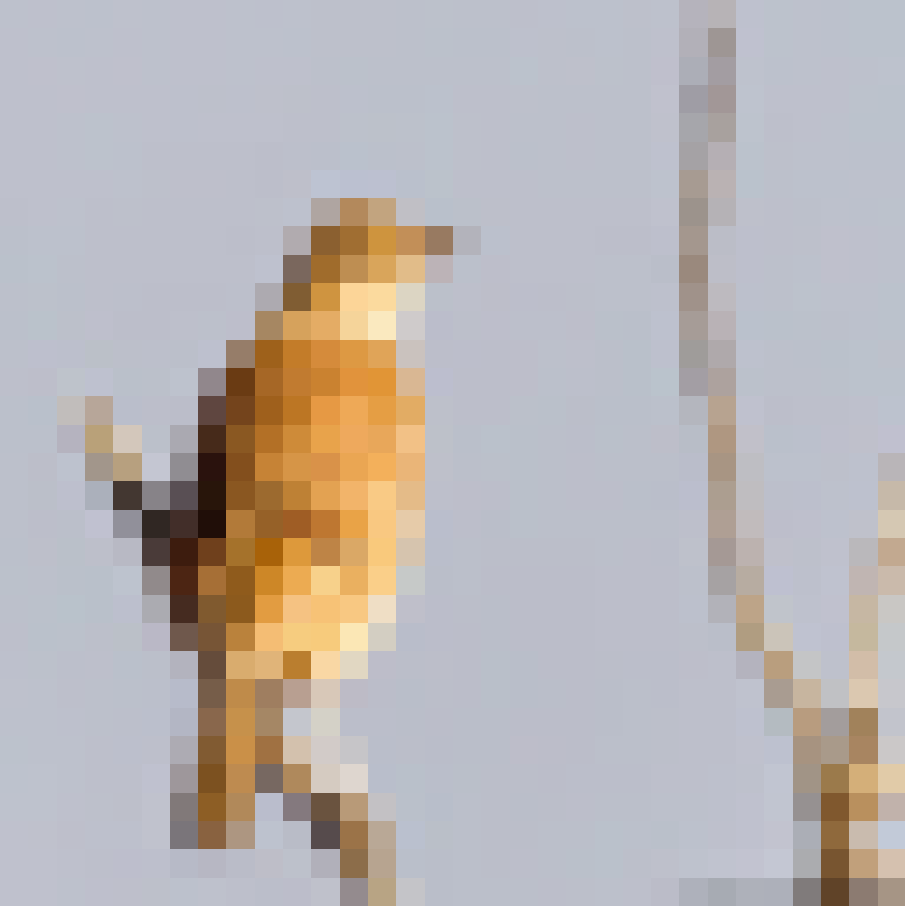
\includegraphics[scale=\scale]{../visualizations/examples/cifar10/cnn/images/2.png} &
%   \includegraphics[scale=\scale]{../visualizations/examples/cifar10/cnn/saliency_map/2.png} & 
%   \includegraphics[scale=\scale]{../visualizations/examples/cifar10/cnn/positive_saliency_map/2.png} & 
%   \includegraphics[scale=\scale]{../visualizations/examples/cifar10/cnn/negative_saliency_map/2.png} & 
%   \includegraphics[scale=\scale]{../visualizations/examples/cifar10/cnn/active_saliency_map/2.png} & 
%   \includegraphics[scale=\scale]{../visualizations/examples/cifar10/cnn/inactive_saliency_map/2.png} \\
  
%   \includegraphics[scale=\scale]{../visualizations/examples/cifar10/cnn/images/3.png} &
%   \includegraphics[scale=\scale]{../visualizations/examples/cifar10/cnn/saliency_map/3.png} & 
%   \includegraphics[scale=\scale]{../visualizations/examples/cifar10/cnn/positive_saliency_map/3.png} & 
%   \includegraphics[scale=\scale]{../visualizations/examples/cifar10/cnn/negative_saliency_map/3.png} & 
%   \includegraphics[scale=\scale]{../visualizations/examples/cifar10/cnn/active_saliency_map/3.png} & 
%   \includegraphics[scale=\scale]{../visualizations/examples/cifar10/cnn/inactive_saliency_map/3.png} \\
  
%   \includegraphics[scale=\scale]{../visualizations/examples/cifar10/cnn/images/4.png} &
%   \includegraphics[scale=\scale]{../visualizations/examples/cifar10/cnn/saliency_map/4.png} & 
%   \includegraphics[scale=\scale]{../visualizations/examples/cifar10/cnn/positive_saliency_map/4.png} & 
%   \includegraphics[scale=\scale]{../visualizations/examples/cifar10/cnn/negative_saliency_map/4.png} & 
%   \includegraphics[scale=\scale]{../visualizations/examples/cifar10/cnn/active_saliency_map/4.png} & 
%   \includegraphics[scale=\scale]{../visualizations/examples/cifar10/cnn/inactive_saliency_map/4.png} \\
  
%   \includegraphics[scale=\scale]{../visualizations/examples/cifar10/cnn/images/5.png} &
%   \includegraphics[scale=\scale]{../visualizations/examples/cifar10/cnn/saliency_map/5.png} & 
%   \includegraphics[scale=\scale]{../visualizations/examples/cifar10/cnn/positive_saliency_map/5.png} & 
%   \includegraphics[scale=\scale]{../visualizations/examples/cifar10/cnn/negative_saliency_map/5.png} & 
%   \includegraphics[scale=\scale]{../visualizations/examples/cifar10/cnn/active_saliency_map/5.png} & 
%   \includegraphics[scale=\scale]{../visualizations/examples/cifar10/cnn/inactive_saliency_map/5.png} \\
  
%   \includegraphics[scale=\scale]{../visualizations/examples/cifar10/cnn/images/6.png} &
%   \includegraphics[scale=\scale]{../visualizations/examples/cifar10/cnn/saliency_map/6.png} & 
%   \includegraphics[scale=\scale]{../visualizations/examples/cifar10/cnn/positive_saliency_map/6.png} & 
%   \includegraphics[scale=\scale]{../visualizations/examples/cifar10/cnn/negative_saliency_map/6.png} & 
%   \includegraphics[scale=\scale]{../visualizations/examples/cifar10/cnn/active_saliency_map/6.png} & 
%   \includegraphics[scale=\scale]{../visualizations/examples/cifar10/cnn/inactive_saliency_map/6.png} \\
  
%   \includegraphics[scale=\scale]{../visualizations/examples/cifar10/cnn/images/7.png} &
%   \includegraphics[scale=\scale]{../visualizations/examples/cifar10/cnn/saliency_map/7.png} & 
%   \includegraphics[scale=\scale]{../visualizations/examples/cifar10/cnn/positive_saliency_map/7.png} & 
%   \includegraphics[scale=\scale]{../visualizations/examples/cifar10/cnn/negative_saliency_map/7.png} & 
%   \includegraphics[scale=\scale]{../visualizations/examples/cifar10/cnn/active_saliency_map/7.png} & 
%   \includegraphics[scale=\scale]{../visualizations/examples/cifar10/cnn/inactive_saliency_map/7.png} \\
  
%   \includegraphics[scale=\scale]{../visualizations/examples/cifar10/cnn/images/8.png} &
%   \includegraphics[scale=\scale]{../visualizations/examples/cifar10/cnn/saliency_map/8.png} & 
%   \includegraphics[scale=\scale]{../visualizations/examples/cifar10/cnn/positive_saliency_map/8.png} & 
%   \includegraphics[scale=\scale]{../visualizations/examples/cifar10/cnn/negative_saliency_map/8.png} & 
%   \includegraphics[scale=\scale]{../visualizations/examples/cifar10/cnn/active_saliency_map/8.png} & 
%   \includegraphics[scale=\scale]{../visualizations/examples/cifar10/cnn/inactive_saliency_map/8.png} \\
  
%   \includegraphics[scale=\scale]{../visualizations/examples/cifar10/cnn/images/9.png} &
%   \includegraphics[scale=\scale]{../visualizations/examples/cifar10/cnn/saliency_map/9.png} & 
%   \includegraphics[scale=\scale]{../visualizations/examples/cifar10/cnn/positive_saliency_map/9.png} & 
%   \includegraphics[scale=\scale]{../visualizations/examples/cifar10/cnn/negative_saliency_map/9.png} & 
%   \includegraphics[scale=\scale]{../visualizations/examples/cifar10/cnn/active_saliency_map/9.png} & 
%   \includegraphics[scale=\scale]{../visualizations/examples/cifar10/cnn/inactive_saliency_map/9.png} \\
%   \end{tabular}
%   \caption{Comparison saliency maps CNN CIFAR-10.}
% \end{figure}

% \begin{figure}[p]
%   \centering
%   \footnotesize
%   \newcommand{\scale}{0.25}
%   \setlength{\tabcolsep}{2pt}
%   \begin{tabular}{cccccc}
%   Image & Original & Positive & Negative & Active & Inactive \\
  
%   \includegraphics[scale=\scale]{../visualizations/examples/cifar10/resnet18/images/0.png} &
%   \includegraphics[scale=\scale]{../visualizations/examples/cifar10/resnet18/saliency_map/0.png} & 
%   \includegraphics[scale=\scale]{../visualizations/examples/cifar10/resnet18/positive_saliency_map/0.png} & 
%   \includegraphics[scale=\scale]{../visualizations/examples/cifar10/resnet18/negative_saliency_map/0.png} & 
%   \includegraphics[scale=\scale]{../visualizations/examples/cifar10/resnet18/active_saliency_map/0.png} & 
%   \includegraphics[scale=\scale]{../visualizations/examples/cifar10/resnet18/inactive_saliency_map/0.png} \\
  
%   \includegraphics[scale=\scale]{../visualizations/examples/cifar10/resnet18/images/1.png} &
%   \includegraphics[scale=\scale]{../visualizations/examples/cifar10/resnet18/saliency_map/1.png} & 
%   \includegraphics[scale=\scale]{../visualizations/examples/cifar10/resnet18/positive_saliency_map/1.png} & 
%   \includegraphics[scale=\scale]{../visualizations/examples/cifar10/resnet18/negative_saliency_map/1.png} & 
%   \includegraphics[scale=\scale]{../visualizations/examples/cifar10/resnet18/active_saliency_map/1.png} & 
%   \includegraphics[scale=\scale]{../visualizations/examples/cifar10/resnet18/inactive_saliency_map/1.png} \\
  
%   \includegraphics[scale=\scale]{../visualizations/examples/cifar10/resnet18/images/2.png} &
%   \includegraphics[scale=\scale]{../visualizations/examples/cifar10/resnet18/saliency_map/2.png} & 
%   \includegraphics[scale=\scale]{../visualizations/examples/cifar10/resnet18/positive_saliency_map/2.png} & 
%   \includegraphics[scale=\scale]{../visualizations/examples/cifar10/resnet18/negative_saliency_map/2.png} & 
%   \includegraphics[scale=\scale]{../visualizations/examples/cifar10/resnet18/active_saliency_map/2.png} & 
%   \includegraphics[scale=\scale]{../visualizations/examples/cifar10/resnet18/inactive_saliency_map/2.png} \\
  
%   \includegraphics[scale=\scale]{../visualizations/examples/cifar10/resnet18/images/3.png} &
%   \includegraphics[scale=\scale]{../visualizations/examples/cifar10/resnet18/saliency_map/3.png} & 
%   \includegraphics[scale=\scale]{../visualizations/examples/cifar10/resnet18/positive_saliency_map/3.png} & 
%   \includegraphics[scale=\scale]{../visualizations/examples/cifar10/resnet18/negative_saliency_map/3.png} & 
%   \includegraphics[scale=\scale]{../visualizations/examples/cifar10/resnet18/active_saliency_map/3.png} & 
%   \includegraphics[scale=\scale]{../visualizations/examples/cifar10/resnet18/inactive_saliency_map/3.png} \\
  
%   \includegraphics[scale=\scale]{../visualizations/examples/cifar10/resnet18/images/4.png} &
%   \includegraphics[scale=\scale]{../visualizations/examples/cifar10/resnet18/saliency_map/4.png} & 
%   \includegraphics[scale=\scale]{../visualizations/examples/cifar10/resnet18/positive_saliency_map/4.png} & 
%   \includegraphics[scale=\scale]{../visualizations/examples/cifar10/resnet18/negative_saliency_map/4.png} & 
%   \includegraphics[scale=\scale]{../visualizations/examples/cifar10/resnet18/active_saliency_map/4.png} & 
%   \includegraphics[scale=\scale]{../visualizations/examples/cifar10/resnet18/inactive_saliency_map/4.png} \\
  
%   \includegraphics[scale=\scale]{../visualizations/examples/cifar10/resnet18/images/5.png} &
%   \includegraphics[scale=\scale]{../visualizations/examples/cifar10/resnet18/saliency_map/5.png} & 
%   \includegraphics[scale=\scale]{../visualizations/examples/cifar10/resnet18/positive_saliency_map/5.png} & 
%   \includegraphics[scale=\scale]{../visualizations/examples/cifar10/resnet18/negative_saliency_map/5.png} & 
%   \includegraphics[scale=\scale]{../visualizations/examples/cifar10/resnet18/active_saliency_map/5.png} & 
%   \includegraphics[scale=\scale]{../visualizations/examples/cifar10/resnet18/inactive_saliency_map/5.png} \\
  
%   \includegraphics[scale=\scale]{../visualizations/examples/cifar10/resnet18/images/6.png} &
%   \includegraphics[scale=\scale]{../visualizations/examples/cifar10/resnet18/saliency_map/6.png} & 
%   \includegraphics[scale=\scale]{../visualizations/examples/cifar10/resnet18/positive_saliency_map/6.png} & 
%   \includegraphics[scale=\scale]{../visualizations/examples/cifar10/resnet18/negative_saliency_map/6.png} & 
%   \includegraphics[scale=\scale]{../visualizations/examples/cifar10/resnet18/active_saliency_map/6.png} & 
%   \includegraphics[scale=\scale]{../visualizations/examples/cifar10/resnet18/inactive_saliency_map/6.png} \\
  
%   \includegraphics[scale=\scale]{../visualizations/examples/cifar10/resnet18/images/7.png} &
%   \includegraphics[scale=\scale]{../visualizations/examples/cifar10/resnet18/saliency_map/7.png} & 
%   \includegraphics[scale=\scale]{../visualizations/examples/cifar10/resnet18/positive_saliency_map/7.png} & 
%   \includegraphics[scale=\scale]{../visualizations/examples/cifar10/resnet18/negative_saliency_map/7.png} & 
%   \includegraphics[scale=\scale]{../visualizations/examples/cifar10/resnet18/active_saliency_map/7.png} & 
%   \includegraphics[scale=\scale]{../visualizations/examples/cifar10/resnet18/inactive_saliency_map/7.png} \\
  
%   \includegraphics[scale=\scale]{../visualizations/examples/cifar10/resnet18/images/8.png} &
%   \includegraphics[scale=\scale]{../visualizations/examples/cifar10/resnet18/saliency_map/8.png} & 
%   \includegraphics[scale=\scale]{../visualizations/examples/cifar10/resnet18/positive_saliency_map/8.png} & 
%   \includegraphics[scale=\scale]{../visualizations/examples/cifar10/resnet18/negative_saliency_map/8.png} & 
%   \includegraphics[scale=\scale]{../visualizations/examples/cifar10/resnet18/active_saliency_map/8.png} & 
%   \includegraphics[scale=\scale]{../visualizations/examples/cifar10/resnet18/inactive_saliency_map/8.png} \\
  
%   \includegraphics[scale=\scale]{../visualizations/examples/cifar10/resnet18/images/9.png} &
%   \includegraphics[scale=\scale]{../visualizations/examples/cifar10/resnet18/saliency_map/9.png} & 
%   \includegraphics[scale=\scale]{../visualizations/examples/cifar10/resnet18/positive_saliency_map/9.png} & 
%   \includegraphics[scale=\scale]{../visualizations/examples/cifar10/resnet18/negative_saliency_map/9.png} & 
%   \includegraphics[scale=\scale]{../visualizations/examples/cifar10/resnet18/active_saliency_map/9.png} & 
%   \includegraphics[scale=\scale]{../visualizations/examples/cifar10/resnet18/inactive_saliency_map/9.png} \\
%   \end{tabular}
%   \caption{Comparison saliency maps ResNet18 CIFAR-10.}
% \end{figure}

% \begin{figure}[p]
%   \centering
%   \footnotesize
%   \newcommand{\scale}{0.25}
%   \setlength{\tabcolsep}{2pt}
%   \begin{tabular}{cccccc}
%   Image & Original & Positive & Negative & Active & Inactive \\
  
%   \includegraphics[scale=\scale]{../visualizations/examples/imagenette/cnn/images/0.png} &
%   \includegraphics[scale=\scale]{../visualizations/examples/imagenette/cnn/saliency_map/0.png} & 
%   \includegraphics[scale=\scale]{../visualizations/examples/imagenette/cnn/positive_saliency_map/0.png} & 
%   \includegraphics[scale=\scale]{../visualizations/examples/imagenette/cnn/negative_saliency_map/0.png} & 
%   \includegraphics[scale=\scale]{../visualizations/examples/imagenette/cnn/active_saliency_map/0.png} & 
%   \includegraphics[scale=\scale]{../visualizations/examples/imagenette/cnn/inactive_saliency_map/0.png} \\
  
%   \includegraphics[scale=\scale]{../visualizations/examples/imagenette/cnn/images/1.png} &
%   \includegraphics[scale=\scale]{../visualizations/examples/imagenette/cnn/saliency_map/1.png} & 
%   \includegraphics[scale=\scale]{../visualizations/examples/imagenette/cnn/positive_saliency_map/1.png} & 
%   \includegraphics[scale=\scale]{../visualizations/examples/imagenette/cnn/negative_saliency_map/1.png} & 
%   \includegraphics[scale=\scale]{../visualizations/examples/imagenette/cnn/active_saliency_map/1.png} & 
%   \includegraphics[scale=\scale]{../visualizations/examples/imagenette/cnn/inactive_saliency_map/1.png} \\
  
%   \includegraphics[scale=\scale]{../visualizations/examples/imagenette/cnn/images/2.png} &
%   \includegraphics[scale=\scale]{../visualizations/examples/imagenette/cnn/saliency_map/2.png} & 
%   \includegraphics[scale=\scale]{../visualizations/examples/imagenette/cnn/positive_saliency_map/2.png} & 
%   \includegraphics[scale=\scale]{../visualizations/examples/imagenette/cnn/negative_saliency_map/2.png} & 
%   \includegraphics[scale=\scale]{../visualizations/examples/imagenette/cnn/active_saliency_map/2.png} & 
%   \includegraphics[scale=\scale]{../visualizations/examples/imagenette/cnn/inactive_saliency_map/2.png} \\
  
%   \includegraphics[scale=\scale]{../visualizations/examples/imagenette/cnn/images/3.png} &
%   \includegraphics[scale=\scale]{../visualizations/examples/imagenette/cnn/saliency_map/3.png} & 
%   \includegraphics[scale=\scale]{../visualizations/examples/imagenette/cnn/positive_saliency_map/3.png} & 
%   \includegraphics[scale=\scale]{../visualizations/examples/imagenette/cnn/negative_saliency_map/3.png} & 
%   \includegraphics[scale=\scale]{../visualizations/examples/imagenette/cnn/active_saliency_map/3.png} & 
%   \includegraphics[scale=\scale]{../visualizations/examples/imagenette/cnn/inactive_saliency_map/3.png} \\
  
%   \includegraphics[scale=\scale]{../visualizations/examples/imagenette/cnn/images/4.png} &
%   \includegraphics[scale=\scale]{../visualizations/examples/imagenette/cnn/saliency_map/4.png} & 
%   \includegraphics[scale=\scale]{../visualizations/examples/imagenette/cnn/positive_saliency_map/4.png} & 
%   \includegraphics[scale=\scale]{../visualizations/examples/imagenette/cnn/negative_saliency_map/4.png} & 
%   \includegraphics[scale=\scale]{../visualizations/examples/imagenette/cnn/active_saliency_map/4.png} & 
%   \includegraphics[scale=\scale]{../visualizations/examples/imagenette/cnn/inactive_saliency_map/4.png} \\
  
%   \includegraphics[scale=\scale]{../visualizations/examples/imagenette/cnn/images/5.png} &
%   \includegraphics[scale=\scale]{../visualizations/examples/imagenette/cnn/saliency_map/5.png} & 
%   \includegraphics[scale=\scale]{../visualizations/examples/imagenette/cnn/positive_saliency_map/5.png} & 
%   \includegraphics[scale=\scale]{../visualizations/examples/imagenette/cnn/negative_saliency_map/5.png} & 
%   \includegraphics[scale=\scale]{../visualizations/examples/imagenette/cnn/active_saliency_map/5.png} & 
%   \includegraphics[scale=\scale]{../visualizations/examples/imagenette/cnn/inactive_saliency_map/5.png} \\
  
%   \includegraphics[scale=\scale]{../visualizations/examples/imagenette/cnn/images/6.png} &
%   \includegraphics[scale=\scale]{../visualizations/examples/imagenette/cnn/saliency_map/6.png} & 
%   \includegraphics[scale=\scale]{../visualizations/examples/imagenette/cnn/positive_saliency_map/6.png} & 
%   \includegraphics[scale=\scale]{../visualizations/examples/imagenette/cnn/negative_saliency_map/6.png} & 
%   \includegraphics[scale=\scale]{../visualizations/examples/imagenette/cnn/active_saliency_map/6.png} & 
%   \includegraphics[scale=\scale]{../visualizations/examples/imagenette/cnn/inactive_saliency_map/6.png} \\
  
%   \includegraphics[scale=\scale]{../visualizations/examples/imagenette/cnn/images/7.png} &
%   \includegraphics[scale=\scale]{../visualizations/examples/imagenette/cnn/saliency_map/7.png} & 
%   \includegraphics[scale=\scale]{../visualizations/examples/imagenette/cnn/positive_saliency_map/7.png} & 
%   \includegraphics[scale=\scale]{../visualizations/examples/imagenette/cnn/negative_saliency_map/7.png} & 
%   \includegraphics[scale=\scale]{../visualizations/examples/imagenette/cnn/active_saliency_map/7.png} & 
%   \includegraphics[scale=\scale]{../visualizations/examples/imagenette/cnn/inactive_saliency_map/7.png} \\
  
%   \includegraphics[scale=\scale]{../visualizations/examples/imagenette/cnn/images/8.png} &
%   \includegraphics[scale=\scale]{../visualizations/examples/imagenette/cnn/saliency_map/8.png} & 
%   \includegraphics[scale=\scale]{../visualizations/examples/imagenette/cnn/positive_saliency_map/8.png} & 
%   \includegraphics[scale=\scale]{../visualizations/examples/imagenette/cnn/negative_saliency_map/8.png} & 
%   \includegraphics[scale=\scale]{../visualizations/examples/imagenette/cnn/active_saliency_map/8.png} & 
%   \includegraphics[scale=\scale]{../visualizations/examples/imagenette/cnn/inactive_saliency_map/8.png} \\
  
%   \includegraphics[scale=\scale]{../visualizations/examples/imagenette/cnn/images/9.png} &
%   \includegraphics[scale=\scale]{../visualizations/examples/imagenette/cnn/saliency_map/9.png} & 
%   \includegraphics[scale=\scale]{../visualizations/examples/imagenette/cnn/positive_saliency_map/9.png} & 
%   \includegraphics[scale=\scale]{../visualizations/examples/imagenette/cnn/negative_saliency_map/9.png} & 
%   \includegraphics[scale=\scale]{../visualizations/examples/imagenette/cnn/active_saliency_map/9.png} & 
%   \includegraphics[scale=\scale]{../visualizations/examples/imagenette/cnn/inactive_saliency_map/9.png} \\
%   \end{tabular}
%   \caption{Comparison saliency maps CNN Imagenette.}
% \end{figure}

% \begin{figure}[p]
%   \centering
%   \footnotesize
%   \newcommand{\scale}{0.25}
%   \setlength{\tabcolsep}{2pt}
%   \begin{tabular}{cccccc}
%   Image & Original & Positive & Negative & Active & Inactive \\
  
%   \includegraphics[scale=\scale]{../visualizations/examples/imagenette/resnet18/images/0.png} &
%   \includegraphics[scale=\scale]{../visualizations/examples/imagenette/resnet18/saliency_map/0.png} & 
%   \includegraphics[scale=\scale]{../visualizations/examples/imagenette/resnet18/positive_saliency_map/0.png} & 
%   \includegraphics[scale=\scale]{../visualizations/examples/imagenette/resnet18/negative_saliency_map/0.png} & 
%   \includegraphics[scale=\scale]{../visualizations/examples/imagenette/resnet18/active_saliency_map/0.png} & 
%   \includegraphics[scale=\scale]{../visualizations/examples/imagenette/resnet18/inactive_saliency_map/0.png} \\
  
%   \includegraphics[scale=\scale]{../visualizations/examples/imagenette/resnet18/images/1.png} &
%   \includegraphics[scale=\scale]{../visualizations/examples/imagenette/resnet18/saliency_map/1.png} & 
%   \includegraphics[scale=\scale]{../visualizations/examples/imagenette/resnet18/positive_saliency_map/1.png} & 
%   \includegraphics[scale=\scale]{../visualizations/examples/imagenette/resnet18/negative_saliency_map/1.png} & 
%   \includegraphics[scale=\scale]{../visualizations/examples/imagenette/resnet18/active_saliency_map/1.png} & 
%   \includegraphics[scale=\scale]{../visualizations/examples/imagenette/resnet18/inactive_saliency_map/1.png} \\
  
%   \includegraphics[scale=\scale]{../visualizations/examples/imagenette/resnet18/images/2.png} &
%   \includegraphics[scale=\scale]{../visualizations/examples/imagenette/resnet18/saliency_map/2.png} & 
%   \includegraphics[scale=\scale]{../visualizations/examples/imagenette/resnet18/positive_saliency_map/2.png} & 
%   \includegraphics[scale=\scale]{../visualizations/examples/imagenette/resnet18/negative_saliency_map/2.png} & 
%   \includegraphics[scale=\scale]{../visualizations/examples/imagenette/resnet18/active_saliency_map/2.png} & 
%   \includegraphics[scale=\scale]{../visualizations/examples/imagenette/resnet18/inactive_saliency_map/2.png} \\
  
%   \includegraphics[scale=\scale]{../visualizations/examples/imagenette/resnet18/images/3.png} &
%   \includegraphics[scale=\scale]{../visualizations/examples/imagenette/resnet18/saliency_map/3.png} & 
%   \includegraphics[scale=\scale]{../visualizations/examples/imagenette/resnet18/positive_saliency_map/3.png} & 
%   \includegraphics[scale=\scale]{../visualizations/examples/imagenette/resnet18/negative_saliency_map/3.png} & 
%   \includegraphics[scale=\scale]{../visualizations/examples/imagenette/resnet18/active_saliency_map/3.png} & 
%   \includegraphics[scale=\scale]{../visualizations/examples/imagenette/resnet18/inactive_saliency_map/3.png} \\
  
%   \includegraphics[scale=\scale]{../visualizations/examples/imagenette/resnet18/images/4.png} &
%   \includegraphics[scale=\scale]{../visualizations/examples/imagenette/resnet18/saliency_map/4.png} & 
%   \includegraphics[scale=\scale]{../visualizations/examples/imagenette/resnet18/positive_saliency_map/4.png} & 
%   \includegraphics[scale=\scale]{../visualizations/examples/imagenette/resnet18/negative_saliency_map/4.png} & 
%   \includegraphics[scale=\scale]{../visualizations/examples/imagenette/resnet18/active_saliency_map/4.png} & 
%   \includegraphics[scale=\scale]{../visualizations/examples/imagenette/resnet18/inactive_saliency_map/4.png} \\
  
%   \includegraphics[scale=\scale]{../visualizations/examples/imagenette/resnet18/images/5.png} &
%   \includegraphics[scale=\scale]{../visualizations/examples/imagenette/resnet18/saliency_map/5.png} & 
%   \includegraphics[scale=\scale]{../visualizations/examples/imagenette/resnet18/positive_saliency_map/5.png} & 
%   \includegraphics[scale=\scale]{../visualizations/examples/imagenette/resnet18/negative_saliency_map/5.png} & 
%   \includegraphics[scale=\scale]{../visualizations/examples/imagenette/resnet18/active_saliency_map/5.png} & 
%   \includegraphics[scale=\scale]{../visualizations/examples/imagenette/resnet18/inactive_saliency_map/5.png} \\
  
%   \includegraphics[scale=\scale]{../visualizations/examples/imagenette/resnet18/images/6.png} &
%   \includegraphics[scale=\scale]{../visualizations/examples/imagenette/resnet18/saliency_map/6.png} & 
%   \includegraphics[scale=\scale]{../visualizations/examples/imagenette/resnet18/positive_saliency_map/6.png} & 
%   \includegraphics[scale=\scale]{../visualizations/examples/imagenette/resnet18/negative_saliency_map/6.png} & 
%   \includegraphics[scale=\scale]{../visualizations/examples/imagenette/resnet18/active_saliency_map/6.png} & 
%   \includegraphics[scale=\scale]{../visualizations/examples/imagenette/resnet18/inactive_saliency_map/6.png} \\
  
%   \includegraphics[scale=\scale]{../visualizations/examples/imagenette/resnet18/images/7.png} &
%   \includegraphics[scale=\scale]{../visualizations/examples/imagenette/resnet18/saliency_map/7.png} & 
%   \includegraphics[scale=\scale]{../visualizations/examples/imagenette/resnet18/positive_saliency_map/7.png} & 
%   \includegraphics[scale=\scale]{../visualizations/examples/imagenette/resnet18/negative_saliency_map/7.png} & 
%   \includegraphics[scale=\scale]{../visualizations/examples/imagenette/resnet18/active_saliency_map/7.png} & 
%   \includegraphics[scale=\scale]{../visualizations/examples/imagenette/resnet18/inactive_saliency_map/7.png} \\
  
%   \includegraphics[scale=\scale]{../visualizations/examples/imagenette/resnet18/images/8.png} &
%   \includegraphics[scale=\scale]{../visualizations/examples/imagenette/resnet18/saliency_map/8.png} & 
%   \includegraphics[scale=\scale]{../visualizations/examples/imagenette/resnet18/positive_saliency_map/8.png} & 
%   \includegraphics[scale=\scale]{../visualizations/examples/imagenette/resnet18/negative_saliency_map/8.png} & 
%   \includegraphics[scale=\scale]{../visualizations/examples/imagenette/resnet18/active_saliency_map/8.png} & 
%   \includegraphics[scale=\scale]{../visualizations/examples/imagenette/resnet18/inactive_saliency_map/8.png} \\
  
%   \includegraphics[scale=\scale]{../visualizations/examples/imagenette/resnet18/images/9.png} &
%   \includegraphics[scale=\scale]{../visualizations/examples/imagenette/resnet18/saliency_map/9.png} & 
%   \includegraphics[scale=\scale]{../visualizations/examples/imagenette/resnet18/positive_saliency_map/9.png} & 
%   \includegraphics[scale=\scale]{../visualizations/examples/imagenette/resnet18/negative_saliency_map/9.png} & 
%   \includegraphics[scale=\scale]{../visualizations/examples/imagenette/resnet18/active_saliency_map/9.png} & 
%   \includegraphics[scale=\scale]{../visualizations/examples/imagenette/resnet18/inactive_saliency_map/9.png} \\
%   \end{tabular}
%   \caption{Comparison saliency maps ResNet18 Imagenette.}
% \end{figure}

%% If you have bibdatabase file and want bibtex to generate the
%% bibitems, please use
%%


%% else use the following coding to input the bibitems directly in the
%% TeX file.

% \begin{thebibliography}{00}

% %% \bibitem{label}
% %% Text of bibliographic item

% \bibitem{}

% \end{thebibliography}
\end{document}
\endinput
%%
%% End of file `elsarticle-template-num.tex'.
